\chapter{Lab 6: Pulse-Width Modulation} \label{day6}

\section{LED dimmer}

The LED dimmer controls the brightness of an LED by manipulating the duty cycle (DC) of the HIGH signal powering the LED. 

\lstinputlisting[language=VHDL]{./L6/E1/src/project_6_1.vhd}

When the counter reaches the DC limit, the PWM signal goes to 0 and does not power the LED anymore. If the counter reaches the limit, it resets the PWM signal to 1 and the counter to 0 and the process starts again. The brightness of the LED is now dependent on the DC: For a low DC, the LED shines dimm and bright for a DC in the order of the maximum value of the counter. Here we chose a counter with a maximum value of 255.

% DC sollte ein 7 bit Vektor mit 6 downto 0 also einem maximalen Wert von 255 sein.

\lstinputlisting[language=VHDL]{./L6/E1/src/project_6_1_tb.vhd}

This testbench enables us to see the progression of the individual variables, signals as well as in- and outputs. The testbench is a very handy debugging tool of the VIVADO editor. Here the editor simulates the code for a given time and with customizable clocks, in- and outputs. 

\begin{figure}[h]
	\centering
	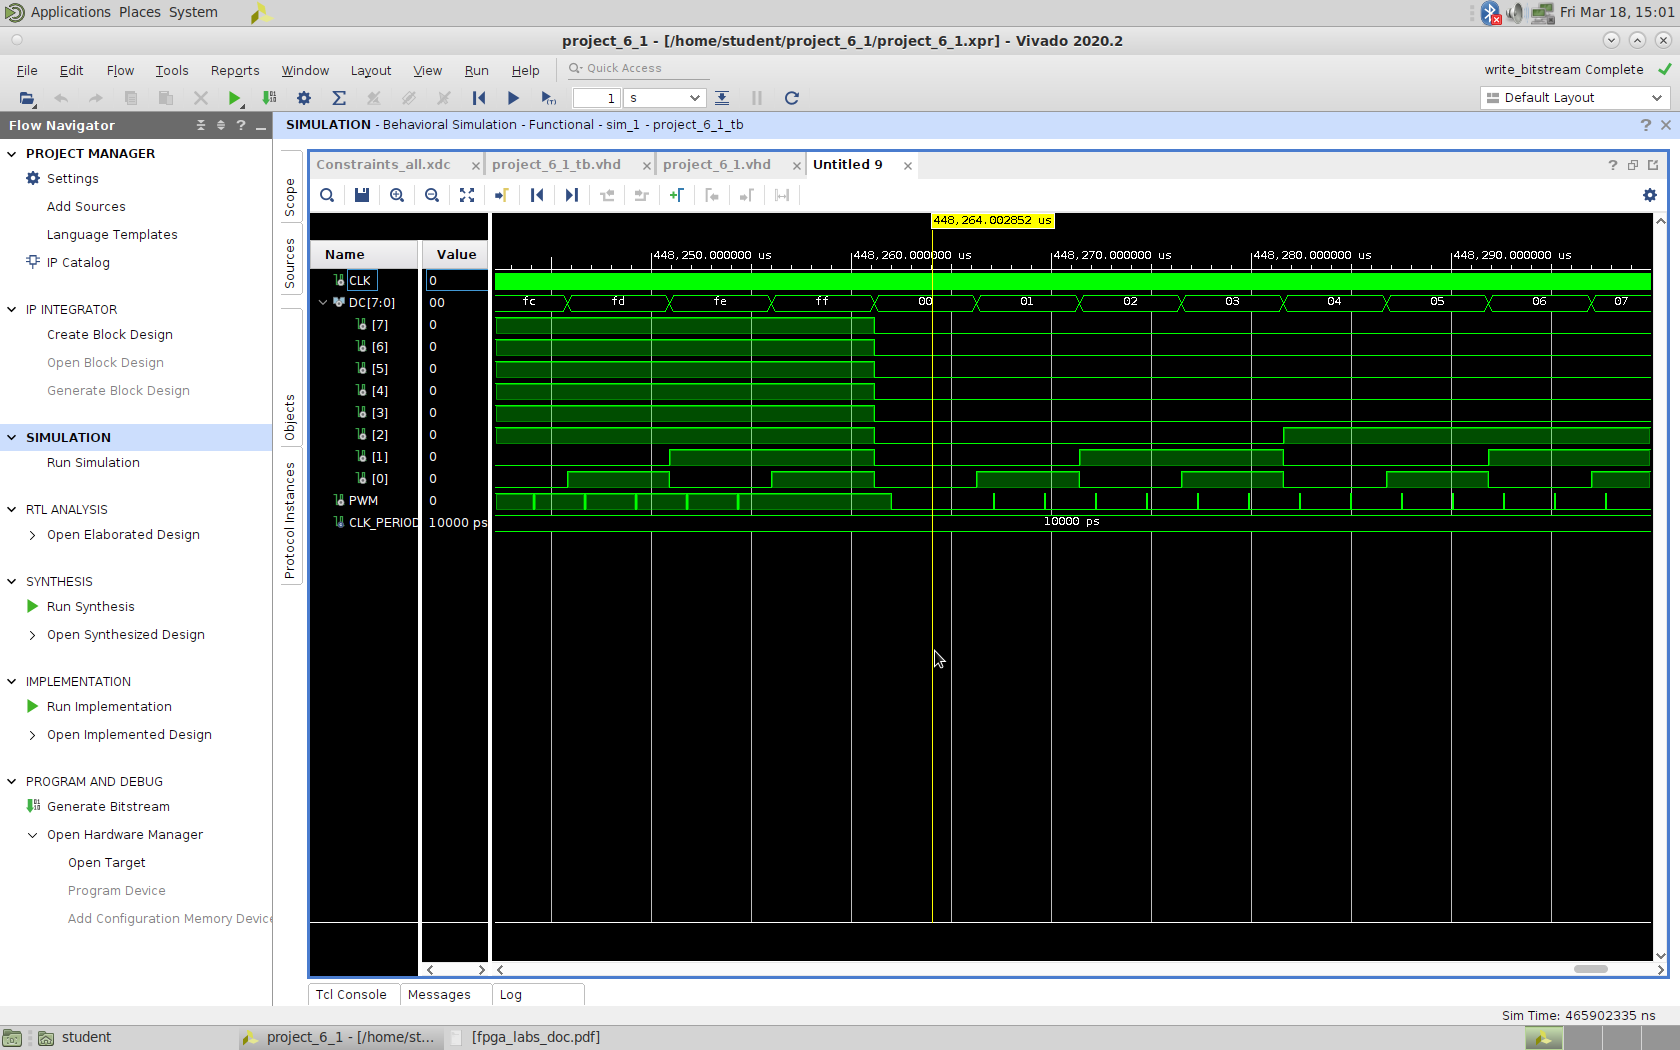
\includegraphics[width=.8\linewidth]{./L6/E1/overflow_time.png}
	\caption{After one full progression the timer is reset to zero.} 
	\label{fig: overflow_time e_6_1 LED dimmer}
\end{figure}

% Wie lange dauert es 1s zu simulieren? Haben wir dazu was aufgeschrieben¿
The simulation takes about 0.5\,s to simulate one second of real time.

\section{Frequency generator}

Next comes a frequency generator. Here, we use the PWM module to generate an audible frequency. Therefore we use a variable frequency and a duty cycle of 50\,\%.

\lstinputlisting[language=VHDL]{./L6/E2/src/project_6_2.vhd}

\lstinputlisting[language=VHDL]{./L6/E2/src/project_6_2_1.vhd}

\lstinputlisting[language=VHDL]{./L6/E2/src/project_6_2_tb.vhd}

After testing the design on the board, we could hear single beats for a frequency of 1\,Hz but we would not consider this a valid sound and the maximum frequency we could hear was between 16000 and 18000\,Hz.

When running the simulation we get a period of 10\,ms for a frequency of 100\,Hz, 1\,ms for 1000\,Hz and 100\,µs for 10000\,Hz. 

\section{Melody}

The following piece of code plays the ``secret'' sound from the ``Legend of Zelda'' games.

\lstinputlisting[language=VHDL]{./L6/E3/src/project_6_3.vhd}

\section{Duty-cycle regulation for a fixed frequency}

Here, we generate a sound with a variable duty cycle and a fixed frequency of 440\,Hz. The variation of the duty cycle enables us to change the speaker volume. The loudest sound can be generated with a duty cycle of 50\,\%. 

% Was haben wir bemerkt als wir die Duty cycle durchgeschaltet haben. Kein linearer Verlauf?

\lstinputlisting[language=VHDL]{./L6/E4/src/project_6_4.vhd}

\lstinputlisting[language=VHDL]{./L6/E4/src/project_6_4_1.vhd}

\section{Duty-cycle regulation for variable frequency}

This program combines the possibility to change the duty cycle and the frequency. Here, we chose to fix the first 6 and last 2 bits of the frequency to 0, so in total the frequency has a range from 128 to 16383\,Hz and 0\,Hz. The duty cycle can be regulated form 0 to 100\,\% with a step size of 1/255 $\approx$ 0.2\,\%.

% auch hier möglicherweise auf 255 ändern

\lstinputlisting[language=VHDL]{./L6/E5/src/project_6_5.vhd}

\lstinputlisting[language=VHDL]{./L6/E5/src/project_6_5_1.vhd}
